% -*- compile-command: "make HOCKING-PeakSegJoint-slides.pdf" -*-
\documentclass{beamer}
\usepackage{tikz}
\usepackage[all]{xy}
\usepackage{amsmath,amssymb}
\usepackage{hyperref}
\usepackage{graphicx}
\usepackage{algorithmic}

\DeclareMathOperator*{\argmin}{arg\,min}
\DeclareMathOperator*{\Lik}{Lik}
\DeclareMathOperator*{\Peaks}{Peaks}
\DeclareMathOperator*{\Segments}{Segments}
\DeclareMathOperator*{\argmax}{arg\,max}
\DeclareMathOperator*{\maximize}{maximize}
\DeclareMathOperator*{\minimize}{minimize}
\newcommand{\sign}{\operatorname{sign}}
\newcommand{\RR}{\mathbb R}
\newcommand{\ZZ}{\mathbb Z}
\newcommand{\NN}{\mathbb N}

% Set transparency of non-highlighted sections in the table of
% contents slide.
\setbeamertemplate{section in toc shaded}[default][100]
\AtBeginSection[]
{
  \setbeamercolor{section in toc}{fg=red} 
  \setbeamercolor{section in toc shaded}{fg=black} 
  \begin{frame}
    \tableofcontents[currentsection]
  \end{frame}
}

\begin{document}

\title{PeakSegJoint: fast supervised peak detection via joint
  segmentation of count data samples}

\author{
  Toby Dylan Hocking\\
  toby.hocking@mail.mcgill.ca\\
  joint work with Guillaume Bourque}

%\date{2 April 2015}

\maketitle

\section{ChIP-seq data and previous work on peak detection}


\begin{frame}
  \frametitle{Chromatin immunoprecipitation sequencing (ChIP-seq)}
  Analysis of DNA-protein interactions.

  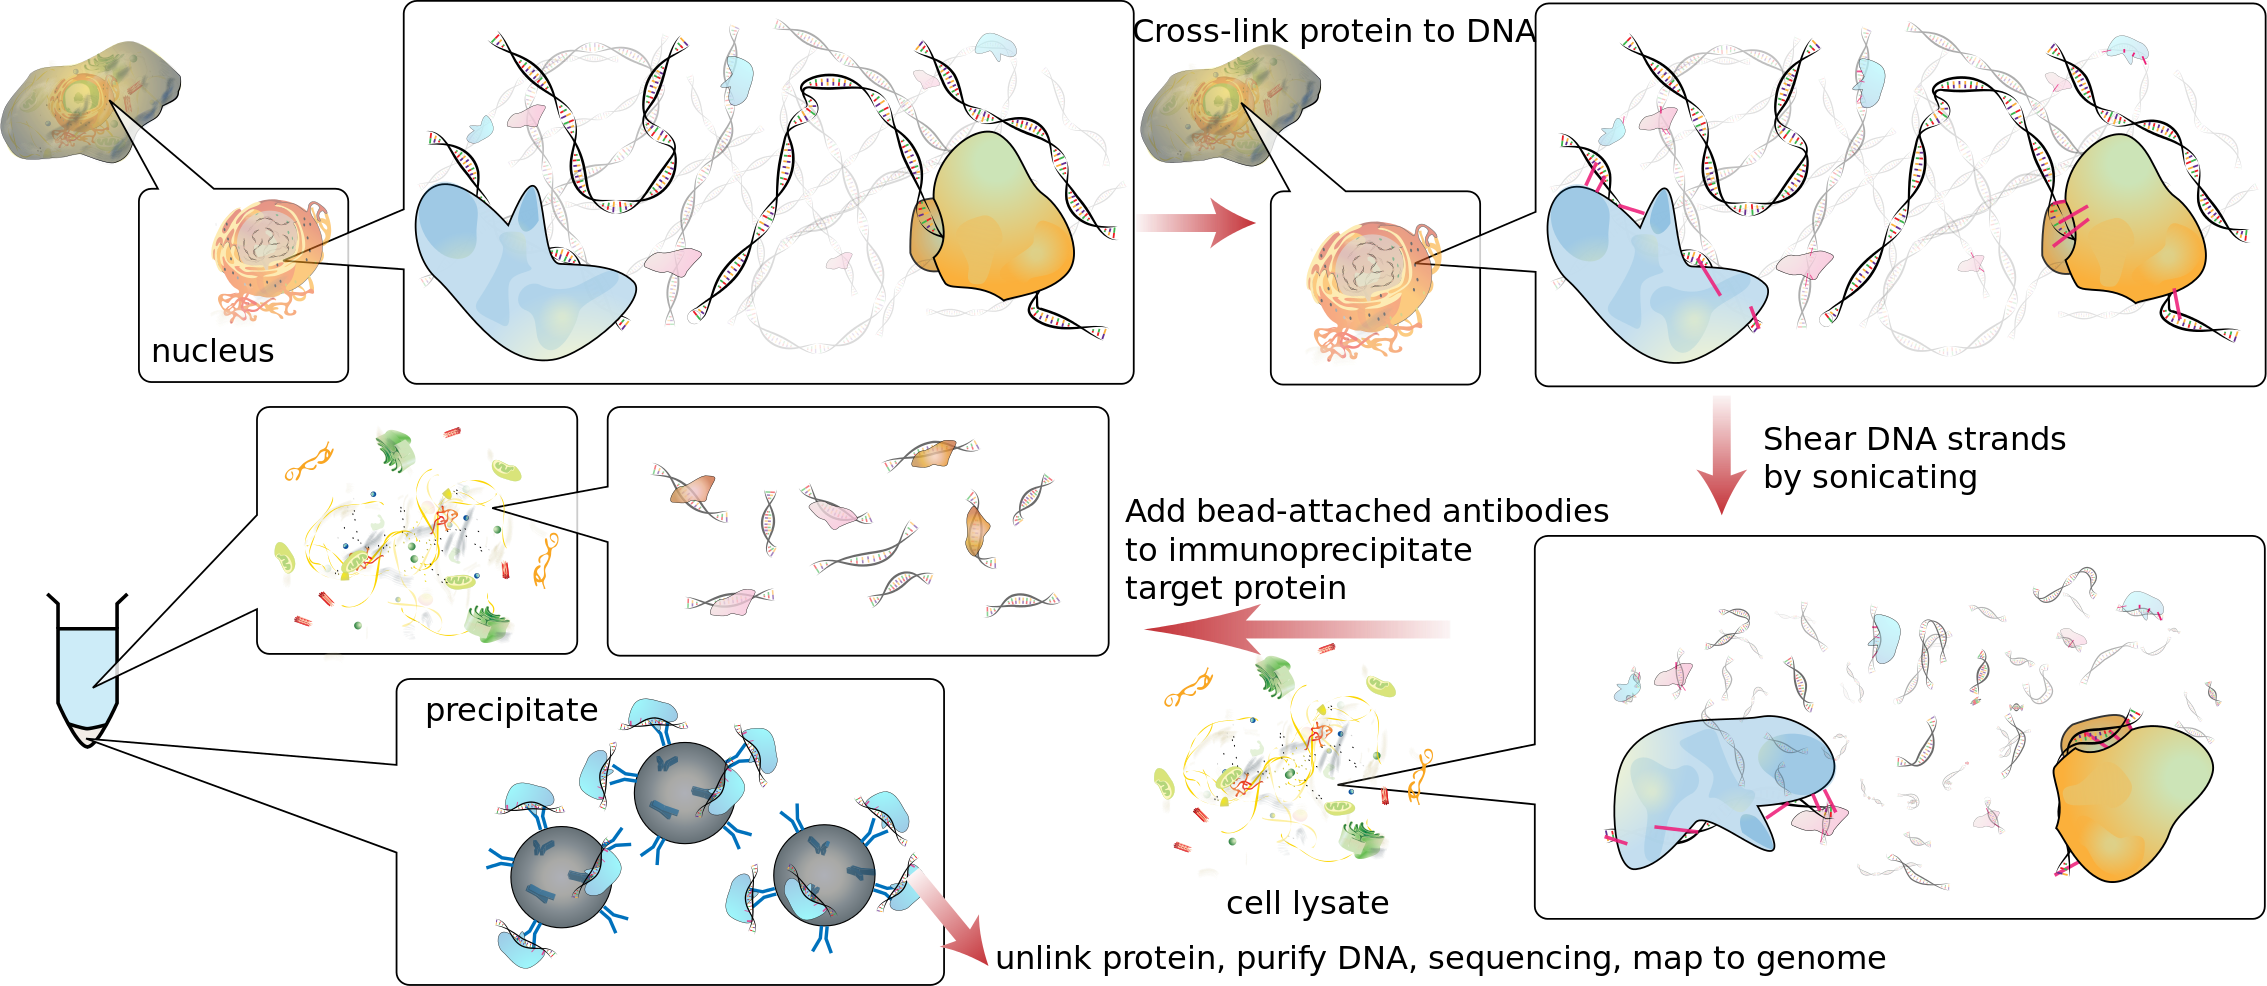
\includegraphics[width=\textwidth]{Chromatin_immunoprecipitation_sequencing_wide.png}

  Source: ``ChIP-sequencing,'' Wikipedia.
\end{frame}

\begin{frame}
  \frametitle{Problem: find peaks in each of several samples}
  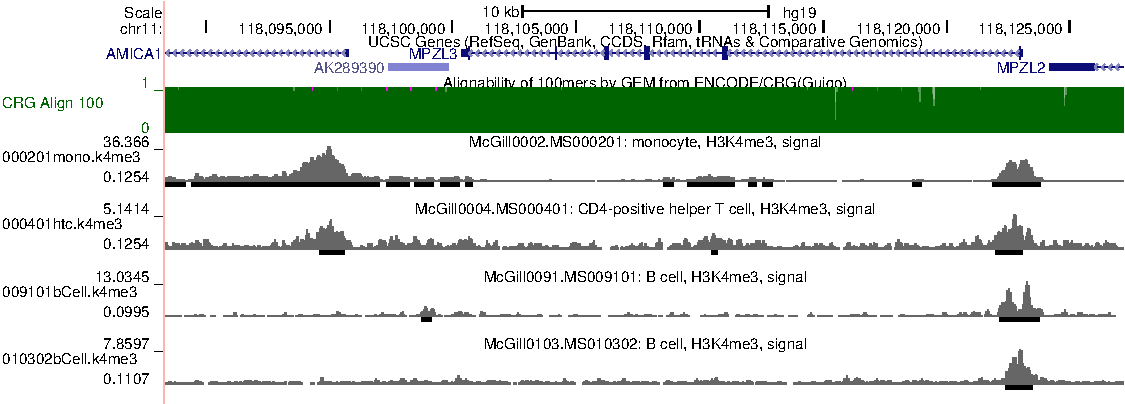
\includegraphics[width=\textwidth]{screenshot-ucsc-edited}

  Grey profiles are normalized aligned read count signals.

  Black bars are ``peaks'' called by MACS2 (Zhang et al, 2008):
  \begin{itemize}
  \item many false positives.
  \item overlapping peaks have different start/end positions.
  \end{itemize}
\end{frame}

\begin{frame}
  \frametitle{Existing peak detection algorithms}
  \begin{itemize}
  \item Model-based analysis of ChIP-Seq (MACS), Zhang et al, 2008.
  \item SICER, Zang et al, 2009.
  \item HOMER findPeaks, Heinz et al, 2010.
  \item RSEG, Song and Smith, 2011.
  \item Histone modifications in cancer (HMCan), Ashoor et al, 2013.
  \item ... dozens of others.
  \end{itemize}
  Two big questions: how to choose the best...
  \begin{itemize}
  \item ...algorithm?
  \item ...parameters?
  \end{itemize}
\end{frame}

\begin{frame}[fragile]
  \frametitle{How to choose parameters of unsupervised peak
    detectors?}
\scriptsize
19 parameters for Model-based analysis of ChIP-Seq (MACS), Zhang et al, 2008.
\begin{verbatim}
  [-g GSIZE]
  [-s TSIZE] [--bw BW] [-m MFOLD MFOLD] [--fix-bimodal]
  [--nomodel] [--extsize EXTSIZE | --shiftsize SHIFTSIZE]
  [-q QVALUE | -p PVALUE | -F FOLDENRICHMENT] [--to-large]
  [--down-sample] [--seed SEED] [--nolambda]
  [--slocal SMALLLOCAL] [--llocal LARGELOCAL]
  [--shift-control] [--half-ext] [--broad]
  [--broad-cutoff BROADCUTOFF] [--call-summits]
\end{verbatim}
10 parameters for Histone modifications in cancer (HMCan),
Ashoor et al, 2013.
\begin{verbatim}
minLength 145
medLength 150
maxLength 155
smallBinLength 50
largeBinLength 100000
pvalueThreshold 0.01
mergeDistance 200
iterationThreshold 5
finalThreshold 0
maxIter 20
\end{verbatim}
\end{frame}

\begin{frame}
  \frametitle{Previous work in computer vision: look and add labels
    to...}
  \begin{tabular}{ccc}
    Photos & Cell images & Copy number profiles \\
    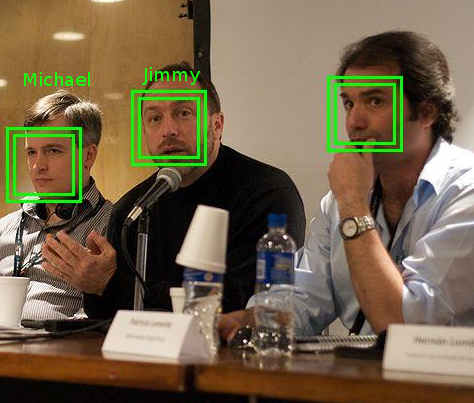
\includegraphics[width=1.3in]{faces} &
    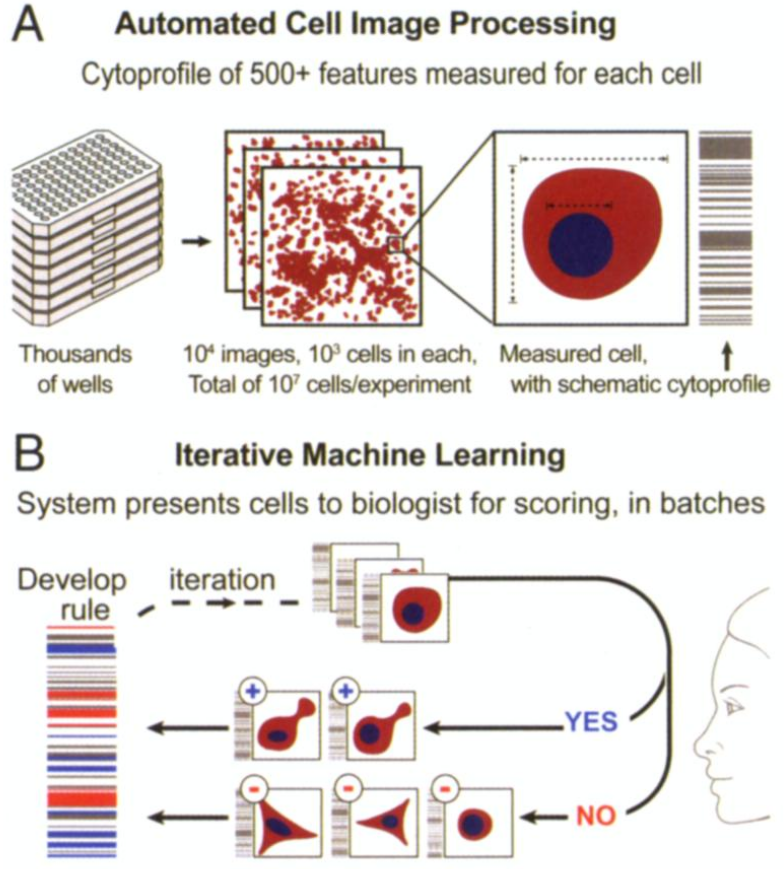
\includegraphics[width=1.3in]{cellprofiler} &
    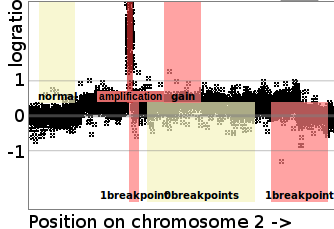
\includegraphics[width=1.5in]{regions-axes}\\
    Labels: names & phenotypes & alterations \\ \\
    CVPR 2013 & CellProfiler & SegAnnDB \\
    246 papers & 873 citations & Hocking et al, 2014. \\
     &
  \end{tabular}
  Sources: \url{http://en.wikipedia.org/wiki/Face_detection}\\
  Jones et al PNAS 2009. Scoring diverse cellular morphologies in
  image-based screens with iterative feedback and machine learning.
\end{frame}

\begin{frame}
  \frametitle{Labels indicate presence/absence of peaks}

  False negative is too few peaks, false positive is too many peaks.

  \includegraphics[width=\textwidth]{figure-good-bad}

  Goals: peaks in same positions across samples,\\
  with minimal number of incorrect regions.

\end{frame}

\begin{frame}
  \frametitle{Goal: minimize number of incorrect labels in test data}
  \begin{itemize}
  \item $S=4$ samples.
  \item $B=50,000$ base positions.
  \item $\mathbf Z \in\ZZ_+^{B\times S}$ matrix of count data.
  \item Set of labels $L$ (peaks, noPeaks, peakStart, peakEnd).
  \item Goal: find a peak caller $c:\ZZ_+^{B\times S} \rightarrow
    \{0,1\}^{B\times S}$ 
  \end{itemize}
  \begin{equation*}
    \label{eq:min_test_err}
    \minimize_c \sum_{i\in\text{test}} E[c(\mathbf Z_i),  L_i],
  \end{equation*}
  where $E$ is the number of incorrect labels\\(false positives + false
  negatives).
\end{frame}

\section{The PeakSeg and PeakSegJoint models} 

\input{figure-profiles-PeakSeg}

\begin{frame}
  \frametitle{PeakSeg: most likely $0, \dots, p_{\text{max}}$ peaks in
    a single sample}

  \begin{itemize}
    \item Count data $\mathbf Z = \left[
    \begin{array}{ccc}
      \mathbf z_1 & \dots & \mathbf z_S
    \end{array}
    \right]\in\ZZ_+^{B\times S}$ for $S$ samples and $B$ bases.
  \item For $p\in\{0, \dots, p_{\text{max}}\}$ peaks, and for each
    sample $\mathbf z\in\ZZ_+^B$, compute the piecewise constant mean
    vector:
  \end{itemize}
  \begin{align*}
    \mathbf{\tilde m}^p(\mathbf z)  =
    \argmin_{\mathbf m\in\RR^{B}} &\ \ 
    \text{PoissonLoss}(\mathbf m, \mathbf z) 
    \\
    \text{such that} &\ \ 
    \Peaks(\mathbf m)=p,  \\
    &\ \  \alert<1>{\forall j\in\{2, \dots, B\},} 
    \ \ \alert<1>{P_j(\mathbf m) \in\{0, 1\}.}\\
    &\ \  \alert<1>{\text{up, down, up, down constraint.}}\\
    %\forall j\in\{1, \dots, B\}, &\ \ P_j(\mathbf m) \in\{0, 1\},
  \end{align*}
  \vskip -1cm
  \begin{itemize}
  \item Peak indicator: $P_j(\mathbf m) = \sum_{k=2}^j \sign( m_{k} - m_{k-1} )$.
  \item Hyper-parameters to choose: genomic window size $B$, maximum
    number of peaks $p_{\text{max}}$.
  \item $O(p_{\text{max}} B^2)$ Constrained Dynamic Programming
    Algorithm (cDPA), Hocking, Rigaill, Bourque, ICML 2015.
  \end{itemize}
\end{frame}

\input{figure-profiles}

\begin{frame}
  \frametitle{PeakSegJoint: best common peak in $0, \dots, S$
    samples}

  \begin{itemize}
  \item $\mathbf Z = \left[
    \begin{array}{ccc}
      \mathbf z_1 & \dots & \mathbf z_S
    \end{array}
  \right]\in\ZZ_+^{B\times S}$ for $B$ bases and $S$ samples.
  \item For $p\in\{0,\dots, S\}$ samples each with 1 common peak,
    compute the mean matrix
  \end{itemize}
\vskip -0.5cm
\begin{align}
  \nonumber \mathbf{\hat M}^p(\mathbf Z)  =
  \argmin_{\mathbf M\in\RR^{B\times S}} &\ \ 
  \sum_{s=1}^S 
  \text{PoissonLoss}(\mathbf m_s, \mathbf z_s) 
  \\
  \text{up, down, up, down:}&\ \nonumber
  \forall s\in\{1, \dots, S\},\,
  \forall j\in\{2, \dots, B\},\\
  &\ P_j(\mathbf m_s) \in\{0, 1\},
  \\
  \text{peaks per sample:} &\ 
  \forall s\in\{1, \dots, S\},\, 
  \Peaks(\mathbf m_s)\in\{0, 1\},  
  \\
  \text{total peaks:}&\ 
  p = \sum_{s=1}^S \Peaks(\mathbf m_s),
  \\
  \text{same starts/ends:} \nonumber &\ \forall s_1\neq s_2\mid
  \Peaks(\mathbf m_{s_1})=\Peaks(\mathbf  m_{s_2})=1,\, \\
   &\ \forall j\in\{1, \dots, B\},\,
  P_j(\mathbf m_{s_1}) = P_j(\mathbf m_{s_2}).
\end{align}

Hocking and Bourque, arXiv:1506.01286.
  
\end{frame}

\section{Fast JointZoom algorithm for approximately solving
  PeakSegJoint}

\begin{frame}
  \frametitle{Comparison of algorithms for Poisson segmentation}

  For $B$ data points to segment,

  \vskip 1cm
  
  \begin{tabular}{ccccc}
    Model & Reference & Algorithm & Time & Exact?\\
    \hline
    Unconstrained & Rigaill  & pDPA & $O(B \log B)$ & Yes. \\
    (no peaks) & arXiv 2010\\
    \hline
    PeakSeg & H et al. & cDPA & $O(B^2)$ & No.\\
    & ICML 2015 \\
    \hline
    PeakSegJoint & H et al. & JointZoom & $O(B\log B)$ & No.\\
    & arXiv 2015
  \end{tabular}
  
\end{frame}

\begin{frame}
  \frametitle{Demonstration of approximate JointZoom algorithm}

  \includegraphics[width=\textwidth]{figure-heuristic-algo}

  Interactive figure at \url{http://bit.ly/1AA6TgK}
\end{frame}

\begin{frame}
  \frametitle{Example runs of approximate JointZoom algorithm}
Previous slide: small data with $B=24$ bases.
\begin{itemize}
\item \textbf{Zoom out} to a bin size of 4 bases.
\item That gives $b=7$ bins.
\item Consider all peak starts/ends = $O(b^2)=15$ models.
\item \textbf{Zoom in} and consider 16 models each at bin sizes 2 and 1.
\end{itemize}
Real data: $B=85846$ bases.
\begin{itemize}
\item Zoom out to a bin size of 16384 bases.
\item That gives $b=6$ bins.
\item Consider all peak starts/ends = $O(b^2)=10$ models.
\item Consider 16 models each at bin sizes 8192, 4096, ..., 4, 2, 1.
\end{itemize}
  Zoom factor parameter fixed at $\beta=2$.
\end{frame}
\begin{frame}
  \frametitle{Time complexity of approximate JointZoom algorithm}

\begin{algorithmic}[1]
  \REQUIRE count data $\mathbf Z\in\ZZ_+^{B\times S}$, zoom factor
  $\beta\in\{2, 3, \dots\}$, number of samples with 1
  peak $p\in\{0, \dots, S\}$.
  \STATE $\textrm{BinSize} \gets \textsc{MaxBinSize}(B, \beta)$. 
  \STATE $\textrm{Peak}, \textrm{Samples} \gets \label{gridsearch}
  \textsc{GridSearch}(\mathbf Z, p, \textrm{BinSize})$.
  \WHILE{$1 < \textrm{BinSize}$}
  \STATE $\textrm{BinSize} \gets \textrm{BinSize} / \beta$. 
  \STATE $\textrm{Peak} \gets
  \textsc{SearchNearPeak}(\mathbf Z, \textrm{Samples}, \label{searchnear}
  \textrm{BinSize}, \textrm{Peak})$
  \ENDWHILE
  \RETURN \textrm{Peak}, \textrm{Samples}.
\end{algorithmic}

\begin{itemize}
\item \textsc{GridSearch} checks $O(1)$ models.
\item Each \textsc{SearchNearPeak} checks $O(\beta^2)$ models.
\item While loop executed $O(\log B)$ times.
\item Computing feasibility and maximum likelihood is $O(pB)$.
\item Time for one model: $O(\beta^2 pB\log B)$.
\item Time for $S+1$ models: $O(\beta^2 S B\log B)$.
\end{itemize}

\end{frame}

\begin{frame}
  \frametitle{PeakSegJoint much faster than other Poisson
    segmentation algorithms}

  Data: simulated single-sample, single-peak.

  \input{figure-timings-small} 

  pDPA from Segmentor3IsBack R package (Cleynen et al, 2014).

  cDPA from PeakSegDP R package (Hocking et al, ICML 2015).

\end{frame}

\section{Speed, train and test error on benchmark data sets}

\begin{frame}
  \frametitle{H3K36me3 data, PeakSeg and Joint model}

  \includegraphics[width=1.1\textwidth]{figure-H3K36me3-profiles}

  \url{http://bl.ocks.org/tdhock/raw/b77c1a7e4d6aee40bf6c/}
\end{frame}

\begin{frame}
  \frametitle{Timings on example H3K36me3 data}

  \small

  Find best 0,...,9 peaks in each of 8 samples (80 PeakSeg
  models):

  \scriptsize

  \input{table-H3K36me3-PeakSeg}

  \vskip 0.2 cm

  \small

  Find best common peak in 0,...,8 samples in each of 5 genomic
  regions (45 PeakSegJoint models):

  \scriptsize

  \input{table-H3K36me3}

\end{frame}

\begin{frame}
  \frametitle{Accuracy benchmark: 7 manually labeled data sets}
  \url{http://cbio.ensmp.fr/~thocking/chip-seq-chunk-db/}
  \begin{itemize}
  \item 4 annotators (AM, TDH, PGP, XJ).
  \item 8 cell types.
  \item 37 annotated H3K4me3 profiles (sharp peak pattern).
  \item 29 annotated H3K36me3 profiles (broad peak pattern).
  \item 12,826 annotated regions in total.
  \item 2752 separate segmentation problems.
  \end{itemize}
  Goal for each data set: divide labels into half train, half test,\\
  then find a peak caller $c:\ZZ_+^{B\times S} \rightarrow
  \{0,1\}^{B\times S}$
  \begin{equation*}
    \minimize_c \sum_{i\in\text{test}} E[c(\mathbf Z_i),  L_i],
  \end{equation*}
  where $E$ is the number of incorrect labels\\(false positives + false
  negatives).
\end{frame}

\begin{frame}
  \frametitle{Train error on H3K4me3 data}
  \includegraphics[width=\textwidth]{../PeakSeg-paper/figure-dp-peaks-train-1}
\end{frame}

\begin{frame}
  \frametitle{Train error on H3K36me3 data}
  \includegraphics[width=\textwidth]{../PeakSeg-paper/figure-dp-peaks-train-2}
\end{frame}

\begin{frame}
  \frametitle{Learned penalty functions for PeakSeg model}

Predicted number of peaks for profile:

\begin{equation*}
  \hat p_i = 
  \argmin_{p}
  \text{PoissonLoss}\left[
    \mathbf{\tilde m}^p(\mathbf z_i),
    \mathbf z_i
  \right]
  + 
  \overbrace{
    \underbrace{\alert<1>{h(p, B_i)}}_{\text{given}}
    \underbrace{\alert<2>{\lambda_i}}_{\text{learned}}
  }^{\text{penalty}},
\end{equation*}

  Names: (model complexity).(number of parameters learned):

  \begin{center}
  \begin{tabular}{ll}
    \textbf{name} & \textbf{model complexity} \alert<1>{$h(p, B_i)$} (not learned) \\
    \hline
    AIC/BIC.* & \alert<1>{$p$}\\
    oracle.* & \alert<1>{$p\left(1 + 4\sqrt{1.1 + \log(B_i/p)}\right)^2$}
  \end{tabular}
\end{center}

  \begin{center}
  \begin{tabular}{lllll}
    \textbf{name} & \textbf{learned} \alert<2>{$\lambda_i = \exp f(\mathbf x_i)$} & 
    \textbf{parameters} & \textbf{learning algo} \\
    \hline
    *.0 & AIC=\alert<2>{2}, BIC=\alert<2>{$\log B_i$} & none & unsupervised \\
    *.1 & 
    \alert<2>{$\beta$} & 
    $\beta\in\RR_+$ & grid search \\
    *.3 & 
    \alert<2>{$e^\beta B_i^{w_1} (\max \mathbf z_i)^{w_{2}}$} & 
    $\beta, w_1, w_{2}\in\RR$ & interval regression \\
    *.41 & 
    \alert<2>{$\exp(\beta + \mathbf w^\intercal \mathbf x_i)$} & 
    $\beta\in\RR, \mathbf w\in\RR^{40}$ & 
    regularized int. reg. \\
  \end{tabular}
\end{center}

\end{frame}

\begin{frame}
  \frametitle{Unsupervised constrained optimization algorithm works
    for both H3K36me3 and H3K4me3 data types}

  ...except in the H3K4me3\_XJ\_immune data set.

  \includegraphics[width=\textwidth]{../PeakSeg-paper/figure-dp-peaks-regression-dots-unsupervised}
  
  Six train/test splits (open circles) and mean (shaded circle).
\end{frame}

\begin{frame}
  \frametitle{Training 1 parameter with grid search reduces test error}

  ...except for macs, good defaults for 3/4 H3K4me3 data sets.

  \includegraphics[width=\textwidth]{../PeakSeg-paper/figure-dp-peaks-regression-dots-grid}

  Six train/test splits (open circles) and mean (shaded circle).
\end{frame}

\begin{frame}
  \frametitle{Training several parameters with interval regression 
    further reduces test error}

  ...except when there are few train data (H3K36me3\_TDH).

  \includegraphics[width=\textwidth]{../PeakSeg-paper/figure-dp-peaks-regression-dots}

  Six train/test splits (open circles) and mean (shaded circle).
\end{frame}


\begin{frame}
  \frametitle{PeakSegJoint error comparable to PeakSeg}

  \includegraphics[width=\textwidth]{figure-test-error-dots.pdf}

  Six train/test splits (open circles) and mean (shaded circle).
\end{frame}

\section{Conclusions}

\begin{frame}[fragile]
  \frametitle{Unsupervised peak detector input: data + parameters}
\scriptsize
19 parameters for Model-based analysis of ChIP-Seq (MACS), Zhang et al, 2008.
\begin{verbatim}
  [-g GSIZE]
  [-s TSIZE] [--bw BW] [-m MFOLD MFOLD] [--fix-bimodal]
  [--nomodel] [--extsize EXTSIZE | --shiftsize SHIFTSIZE]
  [-q QVALUE | -p PVALUE | -F FOLDENRICHMENT] [--to-large]
  [--down-sample] [--seed SEED] [--nolambda]
  [--slocal SMALLLOCAL] [--llocal LARGELOCAL]
  [--shift-control] [--half-ext] [--broad]
  [--broad-cutoff BROADCUTOFF] [--call-summits]
\end{verbatim}
10 parameters for Histone modifications in cancer (HMCan),
Ashoor et al, 2013.
\begin{verbatim}
minLength 145
medLength 150
maxLength 155
smallBinLength 50
largeBinLength 100000
pvalueThreshold 0.01
mergeDistance 200
iterationThreshold 5
finalThreshold 0
maxIter 20
\end{verbatim}
\end{frame}

\begin{frame}
  \frametitle{Supervised peak detector input: data + labels}

  \includegraphics[width=\textwidth]{figure-good-bad}

  Goal: learn a model with minimal incorrect labels on test data.

\end{frame}

\begin{frame}
  \frametitle{Conclusions and future work}
  PeakSeg: \textbf{Peak} detection via constrained optimal
  \textbf{Seg}mentation.\\
  PeakSegJoint: identical overlapping peaks in multiple samples.
  \begin{itemize}
  \item First supervised peak detectors (input = data + labels).
  \item State-of-the-art peak detection for both sharp H3K4me3 and
    broad H3K36me3 profiles.
  \item Oracle model complexity more accurate than AIC/BIC.
  \end{itemize}
  Future work:
  \begin{itemize}
  \item Constrained version of Pruned Dynamic Programming (Rigaill
    arXiv:1004.0887) to compute PeakSeg in $O(B\log B)$ time.
  \item Efficient algorithms for provably computing
    PeakSeg/PeakSegJoint models?
  \item Oracle model complexity for PeakSegJoint \`a la
    Cleynen+Lebarbier?  (2014)
  \item Relaxing the PeakSegJoint 1 peak per sample constraint.
  \end{itemize}
\end{frame}

\begin{frame}
  \frametitle{Thanks for your attention!}
  Write me at \alert{\texttt{toby.hocking@mail.mcgill.ca}} to collaborate!

  \vskip 1cm

  R packages:\\
  \url{https://github.com/tdhock/PeakSegDP}\\
  \url{https://github.com/tdhock/PeakSegJoint}

  \vskip 1cm

  Source code for slides, figures, paper online!\\
  \small
  \url{https://github.com/tdhock/PeakSegJoint-paper}
  \vskip 1cm

  Supplementary slides appear after this one.

\end{frame}

\begin{frame}
  \frametitle{H3K27ac and Input data, PeakSeg and Joint model}

  \includegraphics[width=0.9\textwidth]{figure-H3K27ac-profiles}
\end{frame}

\begin{frame}
  \frametitle{Timings on example H3K27ac data}

  \scriptsize

  \parbox{2in}{
    Find best \\
  0,...,9 peaks\\
  in each of 8 samples\\
  (80 PeakSeg models)

  \input{table-H3K27ac-PeakSeg}
  }
  \parbox{2in}{
  Find best common peak\\
  in 0,...,8 samples\\
  in each of 11 genomic regions\\
  (99 PeakSegJoint models)

  \input{table-H3K27ac}
  }

\end{frame}

\begin{frame}
  \frametitle{H3K4me3 data, PeakSeg and Joint model}

  \includegraphics[width=\textwidth]{figure-H3K4me3-profiles}
\end{frame}

\begin{frame}
  \frametitle{Timings on example H3K4me3 data}

  \small

\parbox{1.5in}{
  Find best \\
  0,...,9 peaks\\
  in each of 10 samples\\
  (100 PeakSeg models)

  \input{table-H3K4me3-PeakSeg}
}
\parbox{2in}{
  Find best common peak\\
  in 0,...,10 samples\\
  in each of 10 genomic regions\\
  (110 PeakSegJoint models)

  \input{table-H3K4me3}
}

\end{frame}

\begin{frame}
  \frametitle{NRSF transcription factor data, PeakSeg and Joint model}

  \includegraphics[width=\textwidth]{figure-nrsf-profiles}
\end{frame}

\begin{frame}
  \frametitle{Timings on example transcription factor data}

  \scriptsize

  Find best \\
  0,...,9 peaks\\
  in each of 4 samples\\
  (40 PeakSeg models)

  \input{table-nrsf-PeakSeg}

  \vskip 0.2cm

  Find best common peak\\
  in 0,...,4 samples\\
  in each of 5 genomic regions\\
  (25 PeakSegJoint models)

  \input{table-nrsf}

\end{frame}

\begin{frame}
  \frametitle{Bin factor parameter controls optimality and speed}
  \includegraphics[width=\textwidth]{figure-bin-factor}

  H3K36me3 example data set, PeakSegJoint model with 2 peaks.
\end{frame}

\begin{frame}
  \frametitle{H3K36me3 data, cDPA and heuristic algorithms}

  \includegraphics[width=\textwidth]{figure-heuristic-profiles}
\end{frame}

\begin{frame}
  \frametitle{Heuristic is much faster than cDPA}

  \includegraphics[height=0.9\textheight]{figure-heuristic-times}
\end{frame}

\begin{frame}
  \frametitle{Heuristic often as good as cDPA}

  \includegraphics[height=0.9\textheight]{figure-heuristic-loss}
\end{frame}


\begin{frame}
  \frametitle{Weighted train error not good for model selection}

  \includegraphics[height=0.9\textheight]{figure-weighted-error}
\end{frame}

\begin{frame}
  \frametitle{Select L1-regularized model with minimal validation error}

  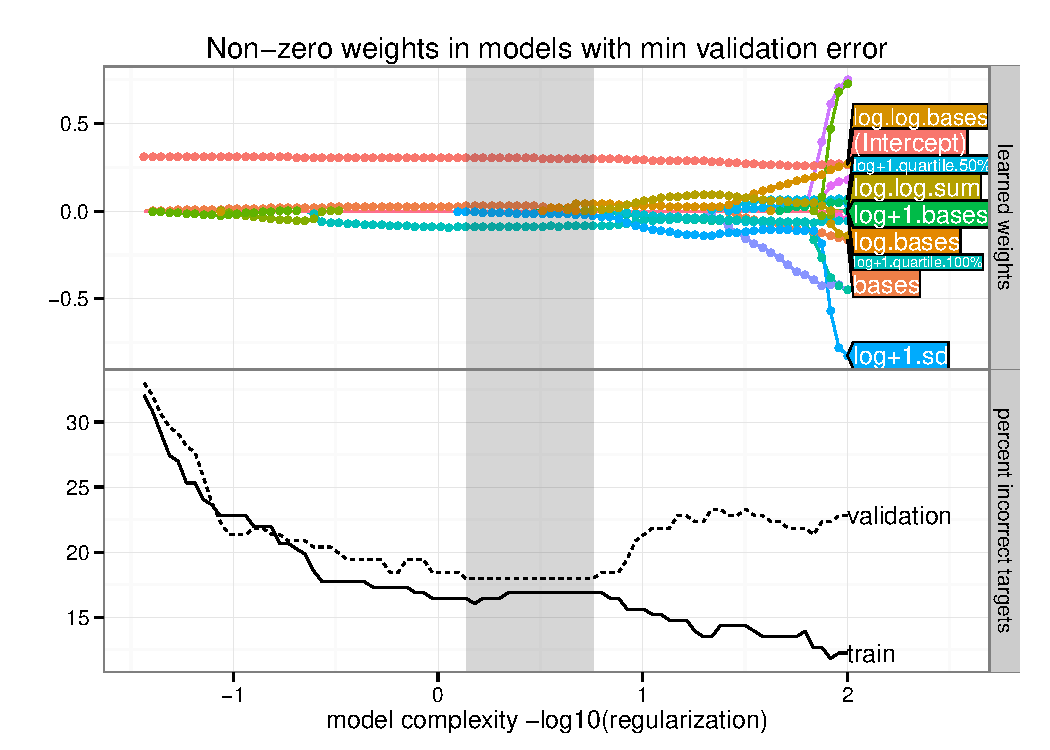
\includegraphics[height=0.9\textheight]{figure-lasso-path}
\end{frame}

\end{document}
